\chapter{Inspect Profunctor Page Artifacts}\label{record-025}

\noindent{\footnotesize\color{BookMuted}\path{docs/reference/profunctor-page-inspection.md}\par}\smallskip

Use \texttt{l\allowbreak{}o\allowbreak{}w\allowbreak{}e\allowbreak{}r\allowbreak{}P\allowbreak{}r\allowbreak{}o\allowbreak{}f\allowbreak{}u\allowbreak{}n\allowbreak{}c\allowbreak{}t\allowbreak{}o\allowbreak{}r\allowbreak{}P\allowbreak{}a\allowbreak{}g\allowbreak{}e\allowbreak{}A\allowbreak{}r\allowbreak{}t\allowbreak{}i\allowbreak{}f\allowbreak{}a\allowbreak{}c\allowbreak{}t\allowbreak{}s\allowbreak{}(\allowbreak{})} to validate and inspect one canonical Profunctor Page artifact family through Bijou's terminal target. The function returns a deterministic \texttt{u\allowbreak{}i\allowbreak{}-\allowbreak{}s\allowbreak{}c\allowbreak{}e\allowbreak{}n\allowbreak{}e\allowbreak{}-\allowbreak{}i\allowbreak{}r\allowbreak{}/\allowbreak{}1} scene, \texttt{S\allowbreak{}u\allowbreak{}r\allowbreak{}f\allowbreak{}a\allowbreak{}c\allowbreak{}e}, target map, receipt, and text witness. It does not mutate the input artifacts.

This reference covers the bounded \texttt{b\allowbreak{}i\allowbreak{}j\allowbreak{}o\allowbreak{}u\allowbreak{}-\allowbreak{}t\allowbreak{}e\allowbreak{}r\allowbreak{}m\allowbreak{}i\allowbreak{}n\allowbreak{}a\allowbreak{}l\allowbreak{}-\allowbreak{}p\allowbreak{}r\allowbreak{}o\allowbreak{}j\allowbreak{}e\allowbreak{}c\allowbreak{}t\allowbreak{}-\allowbreak{}p\allowbreak{}a\allowbreak{}g\allowbreak{}e\allowbreak{}/\allowbreak{}1} target. It is not a general Profunctor Page renderer.

\section{Public API}\label{record-025-public-api}

Import the function, error type, and input or output types from \texttt{@\allowbreak{}f\allowbreak{}l\allowbreak{}y\allowbreak{}i\allowbreak{}n\allowbreak{}g\allowbreak{}r\allowbreak{}o\allowbreak{}b\allowbreak{}o\allowbreak{}t\allowbreak{}s\allowbreak{}/\allowbreak{}b\allowbreak{}i\allowbreak{}j\allowbreak{}o\allowbreak{}u}:

\begin{CodeBlock}
import {
  lowerProfunctorPageArtifacts,
  ProfunctorPageTargetError,
  type ProfunctorArtifactInputs,
  type ProfunctorPageInspectionMode,
  type ProfunctorPageTargetProof,
} from '@flyingrobots/bijou';
\end{CodeBlock}

The call accepts three exact UTF-8 JSON sources:

\begin{CodeBlock}
const inputs: ProfunctorArtifactInputs = {
  page: {
    filename: 'page.profunctor.json',
    source: pageSource,
  },
  sourceMap: {
    filename: 'page.profunctor.map.json',
    source: sourceMapSource,
  },
  buildManifest: {
    filename: 'page.profunctor.build.json',
    source: buildManifestSource,
  },
};

const proof: ProfunctorPageTargetProof =
  lowerProfunctorPageArtifacts(inputs, { mode: 'source-refs' });
\end{CodeBlock}

The example is illustrative. \texttt{p\allowbreak{}a\allowbreak{}g\allowbreak{}e\allowbreak{}S\allowbreak{}o\allowbreak{}u\allowbreak{}r\allowbreak{}c\allowbreak{}e}, \texttt{s\allowbreak{}o\allowbreak{}u\allowbreak{}r\allowbreak{}c\allowbreak{}e\allowbreak{}M\allowbreak{}a\allowbreak{}p\allowbreak{}S\allowbreak{}o\allowbreak{}u\allowbreak{}r\allowbreak{}c\allowbreak{}e}, and \texttt{b\allowbreak{}u\allowbreak{}i\allowbreak{}l\allowbreak{}d\allowbreak{}M\allowbreak{}a\allowbreak{}n\allowbreak{}i\allowbreak{}f\allowbreak{}e\allowbreak{}s\allowbreak{}t\allowbreak{}S\allowbreak{}o\allowbreak{}u\allowbreak{}r\allowbreak{}c\allowbreak{}e} must contain the complete canonical artifact bytes.

\section{Inputs}\label{record-025-inputs}

\begin{center}
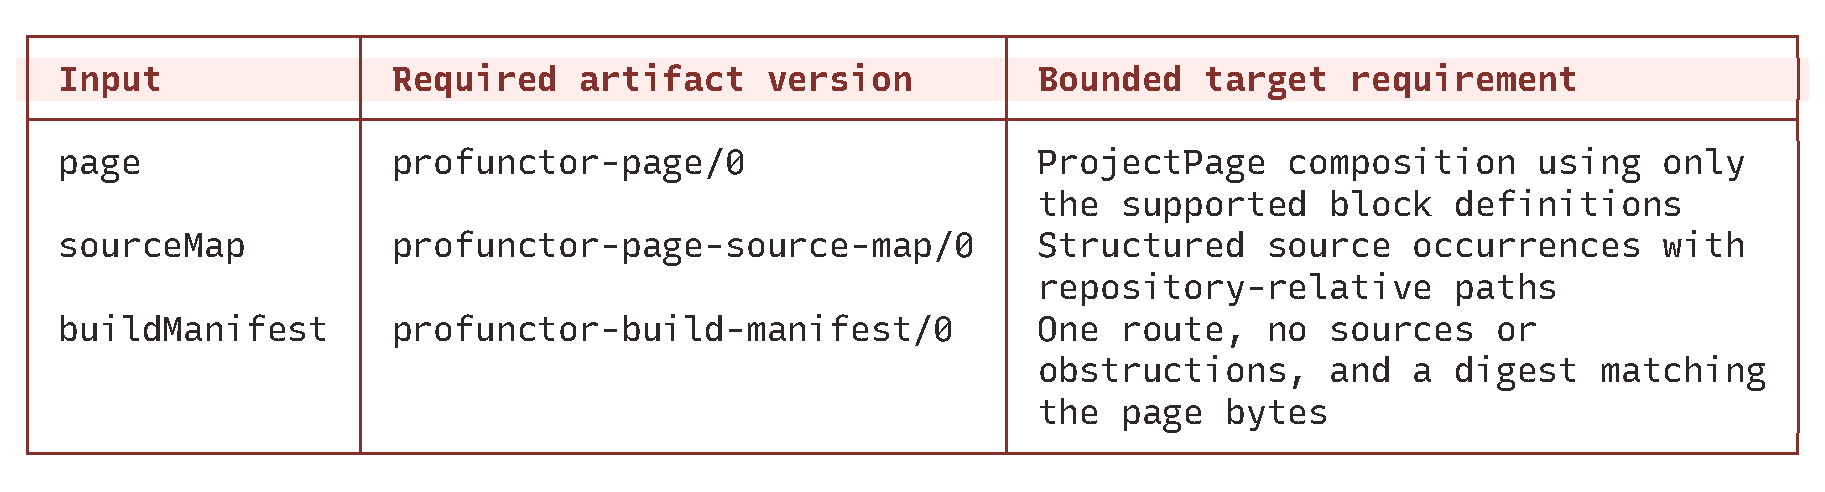
\includegraphics[width=\linewidth]{figures/tables/table-012-g1-1.pdf}
\par\smallskip{\scriptsize\color{BookMuted}Rows 1–3. Actual Bijou table component.}
\end{center}


Each source must be canonical JSON with either no trailing newline or exactly one trailing newline. The parser rejects unknown fields, missing fields, duplicate identities, malformed identity prefixes, host-local paths, digest drift, and cross-artifact disagreement.

The page, source map, and build manifest must agree on the page identity. The manifest entity must agree with the page entity, its sole route must equal the page route, and its dependencies must equal the page dependency digests in the same order. Every source-map source and record digest, node provenance source digest, and build entity digest must occur in that dependency list. The page root must be a visible \texttt{b\allowbreak{}l\allowbreak{}o\allowbreak{}c\allowbreak{}k\allowbreak{}:\allowbreak{}p\allowbreak{}a\allowbreak{}g\allowbreak{}e} whose route agrees with the page route. It must appear first in reading order, and every page node must be reachable from it through the declared slots.

\section{Supported Blocks}\label{record-025-supported-blocks}

The bounded target supports these visible block definitions:

\begin{itemize}
\tightlist
\item
  \texttt{b\allowbreak{}l\allowbreak{}o\allowbreak{}c\allowbreak{}k\allowbreak{}:\allowbreak{}p\allowbreak{}a\allowbreak{}g\allowbreak{}e}
\item
  \texttt{b\allowbreak{}l\allowbreak{}o\allowbreak{}c\allowbreak{}k\allowbreak{}:\allowbreak{}p\allowbreak{}r\allowbreak{}o\allowbreak{}j\allowbreak{}e\allowbreak{}c\allowbreak{}t\allowbreak{}-\allowbreak{}h\allowbreak{}e\allowbreak{}r\allowbreak{}o}
\item
  \texttt{b\allowbreak{}l\allowbreak{}o\allowbreak{}c\allowbreak{}k\allowbreak{}:\allowbreak{}p\allowbreak{}r\allowbreak{}o\allowbreak{}j\allowbreak{}e\allowbreak{}c\allowbreak{}t\allowbreak{}-\allowbreak{}f\allowbreak{}a\allowbreak{}c\allowbreak{}t\allowbreak{}s}
\item
  \texttt{b\allowbreak{}l\allowbreak{}o\allowbreak{}c\allowbreak{}k\allowbreak{}:\allowbreak{}p\allowbreak{}r\allowbreak{}o\allowbreak{}j\allowbreak{}e\allowbreak{}c\allowbreak{}t\allowbreak{}-\allowbreak{}d\allowbreak{}o\allowbreak{}c\allowbreak{}u\allowbreak{}m\allowbreak{}e\allowbreak{}n\allowbreak{}t\allowbreak{}a\allowbreak{}t\allowbreak{}i\allowbreak{}o\allowbreak{}n}
\item
  \texttt{b\allowbreak{}l\allowbreak{}o\allowbreak{}c\allowbreak{}k\allowbreak{}:\allowbreak{}p\allowbreak{}r\allowbreak{}o\allowbreak{}j\allowbreak{}e\allowbreak{}c\allowbreak{}t\allowbreak{}-\allowbreak{}r\allowbreak{}e\allowbreak{}l\allowbreak{}a\allowbreak{}t\allowbreak{}e\allowbreak{}d}
\end{itemize}

A visible unsupported block fails with \texttt{B\allowbreak{}I\allowbreak{}J\allowbreak{}O\allowbreak{}U\allowbreak{}\_\allowbreak{}P\allowbreak{}A\allowbreak{}G\allowbreak{}E\allowbreak{}\_\allowbreak{}B\allowbreak{}L\allowbreak{}O\allowbreak{}C\allowbreak{}K\allowbreak{}\_\allowbreak{}U\allowbreak{}N\allowbreak{}S\allowbreak{}U\allowbreak{}P\allowbreak{}P\allowbreak{}O\allowbreak{}R\allowbreak{}T\allowbreak{}E\allowbreak{}D}. A hidden unsupported block becomes an explicit \texttt{h\allowbreak{}i\allowbreak{}d\allowbreak{}d\allowbreak{}e\allowbreak{}n\allowbreak{}-\allowbreak{}u\allowbreak{}n\allowbreak{}s\allowbreak{}u\allowbreak{}p\allowbreak{}p\allowbreak{}o\allowbreak{}r\allowbreak{}t\allowbreak{}e\allowbreak{}d\allowbreak{}-\allowbreak{}b\allowbreak{}l\allowbreak{}o\allowbreak{}c\allowbreak{}k} residual. Content that cannot fit the bounded 100-column by 28-row terminal profile also fails instead of being clipped.

Semantic-document source-map entries, build-manifest document sources, and application islands are outside this target. They fail explicitly instead of being approximated.

\section{Inspection Modes}\label{record-025-inspection-modes}

Omit \texttt{m\allowbreak{}o\allowbreak{}d\allowbreak{}e} to use \texttt{n\allowbreak{}o\allowbreak{}r\allowbreak{}m\allowbreak{}a\allowbreak{}l}.

\begin{center}
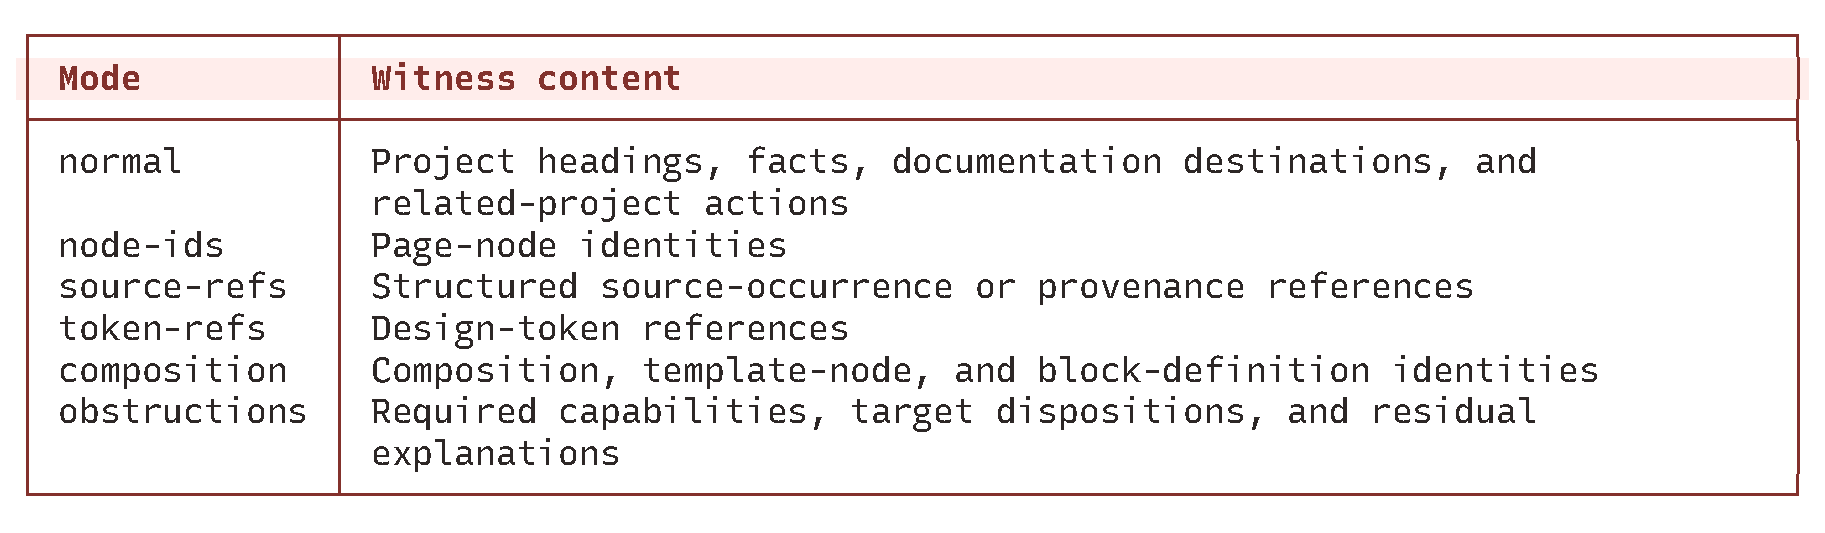
\includegraphics[width=\linewidth]{figures/tables/table-013-g1-1.pdf}
\par\smallskip{\scriptsize\color{BookMuted}Rows 1–6. Actual Bijou table component.}
\end{center}


Modes change the terminal witness. They do not change the input identities or claim browser semantics. Unsupported modes and unowned option fields fail with \texttt{B\allowbreak{}I\allowbreak{}J\allowbreak{}O\allowbreak{}U\allowbreak{}\_\allowbreak{}P\allowbreak{}A\allowbreak{}G\allowbreak{}E\allowbreak{}\_\allowbreak{}I\allowbreak{}N\allowbreak{}P\allowbreak{}U\allowbreak{}T\allowbreak{}\_\allowbreak{}R\allowbreak{}E\allowbreak{}F\allowbreak{}E\allowbreak{}R\allowbreak{}E\allowbreak{}N\allowbreak{}C\allowbreak{}E\allowbreak{}\_\allowbreak{}I\allowbreak{}N\allowbreak{}V\allowbreak{}A\allowbreak{}L\allowbreak{}I\allowbreak{}D}. Multi-value diagnostic facts use one bounded terminal row per value so the witness preserves every fact.

\section{Outputs}\label{record-025-outputs}

\texttt{P\allowbreak{}r\allowbreak{}o\allowbreak{}f\allowbreak{}u\allowbreak{}n\allowbreak{}c\allowbreak{}t\allowbreak{}o\allowbreak{}r\allowbreak{}P\allowbreak{}a\allowbreak{}g\allowbreak{}e\allowbreak{}T\allowbreak{}a\allowbreak{}r\allowbreak{}g\allowbreak{}e\allowbreak{}t\allowbreak{}P\allowbreak{}r\allowbreak{}o\allowbreak{}o\allowbreak{}f} contains:

\begin{center}
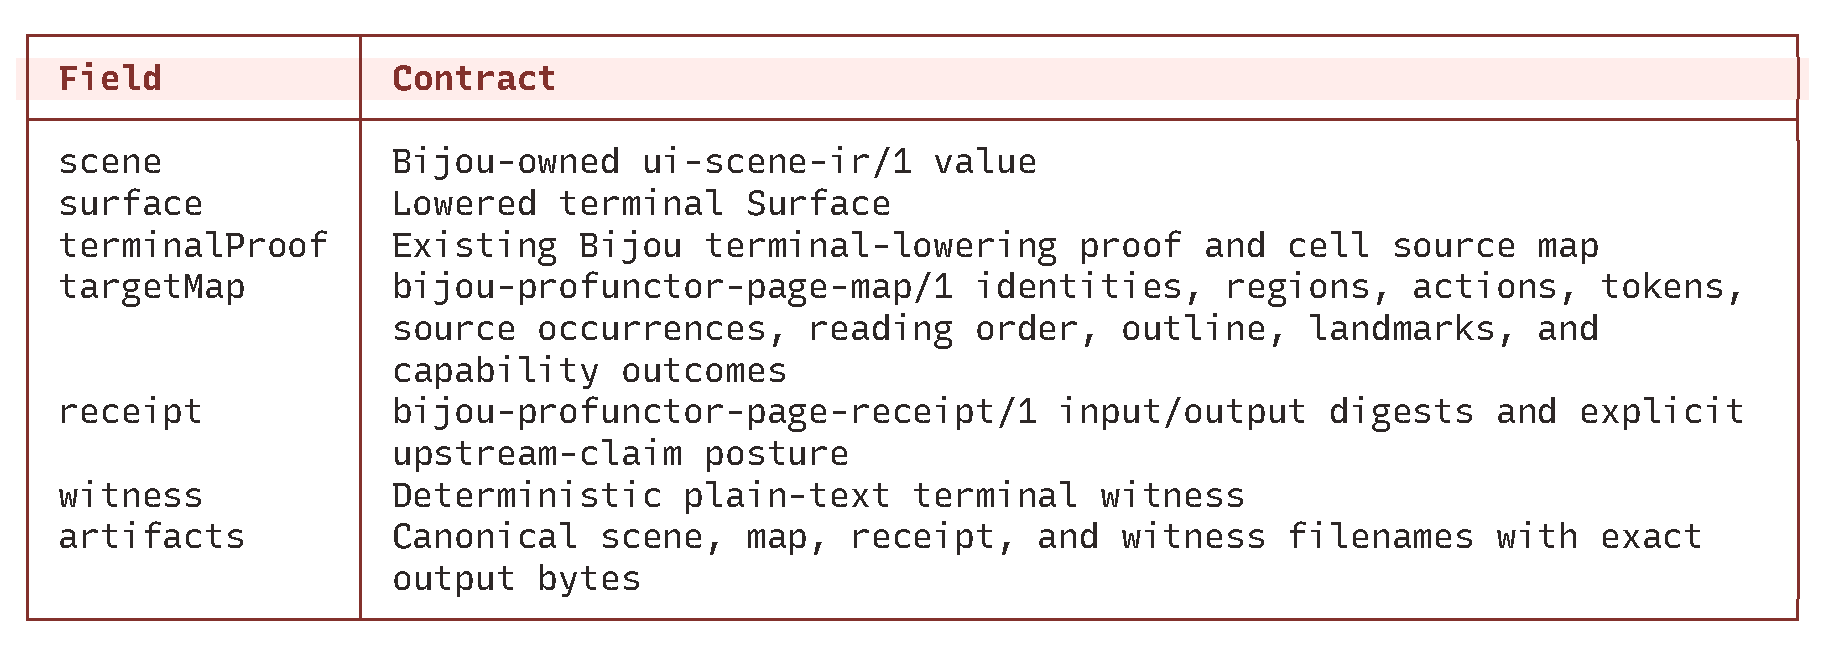
\includegraphics[width=\linewidth]{figures/tables/table-014-g1-1.pdf}
\par\smallskip{\scriptsize\color{BookMuted}Rows 1–7. Actual Bijou table component.}
\end{center}


The target preserves page, composition, override, template, content, source-occurrence, token, action, and target-render identities. Every visible page node receives one render identity. A hidden unsupported node receives one explicit residual.

Native links become Bijou action facts. Heading and landmark semantics become structural facts. Semantic HTML remains an explicit residual; the target does not inherit the build manifest's browser claims.

\section{Diagnostics}\label{record-025-diagnostics}

Failures throw \texttt{P\allowbreak{}r\allowbreak{}o\allowbreak{}f\allowbreak{}u\allowbreak{}n\allowbreak{}c\allowbreak{}t\allowbreak{}o\allowbreak{}r\allowbreak{}P\allowbreak{}a\allowbreak{}g\allowbreak{}e\allowbreak{}T\allowbreak{}a\allowbreak{}r\allowbreak{}g\allowbreak{}e\allowbreak{}t\allowbreak{}E\allowbreak{}r\allowbreak{}r\allowbreak{}o\allowbreak{}r}. Inspect \texttt{c\allowbreak{}o\allowbreak{}d\allowbreak{}e}, \texttt{p\allowbreak{}a\allowbreak{}t\allowbreak{}h}, and \texttt{d\allowbreak{}e\allowbreak{}t\allowbreak{}a\allowbreak{}i\allowbreak{}l} instead of parsing the message.

\begin{center}
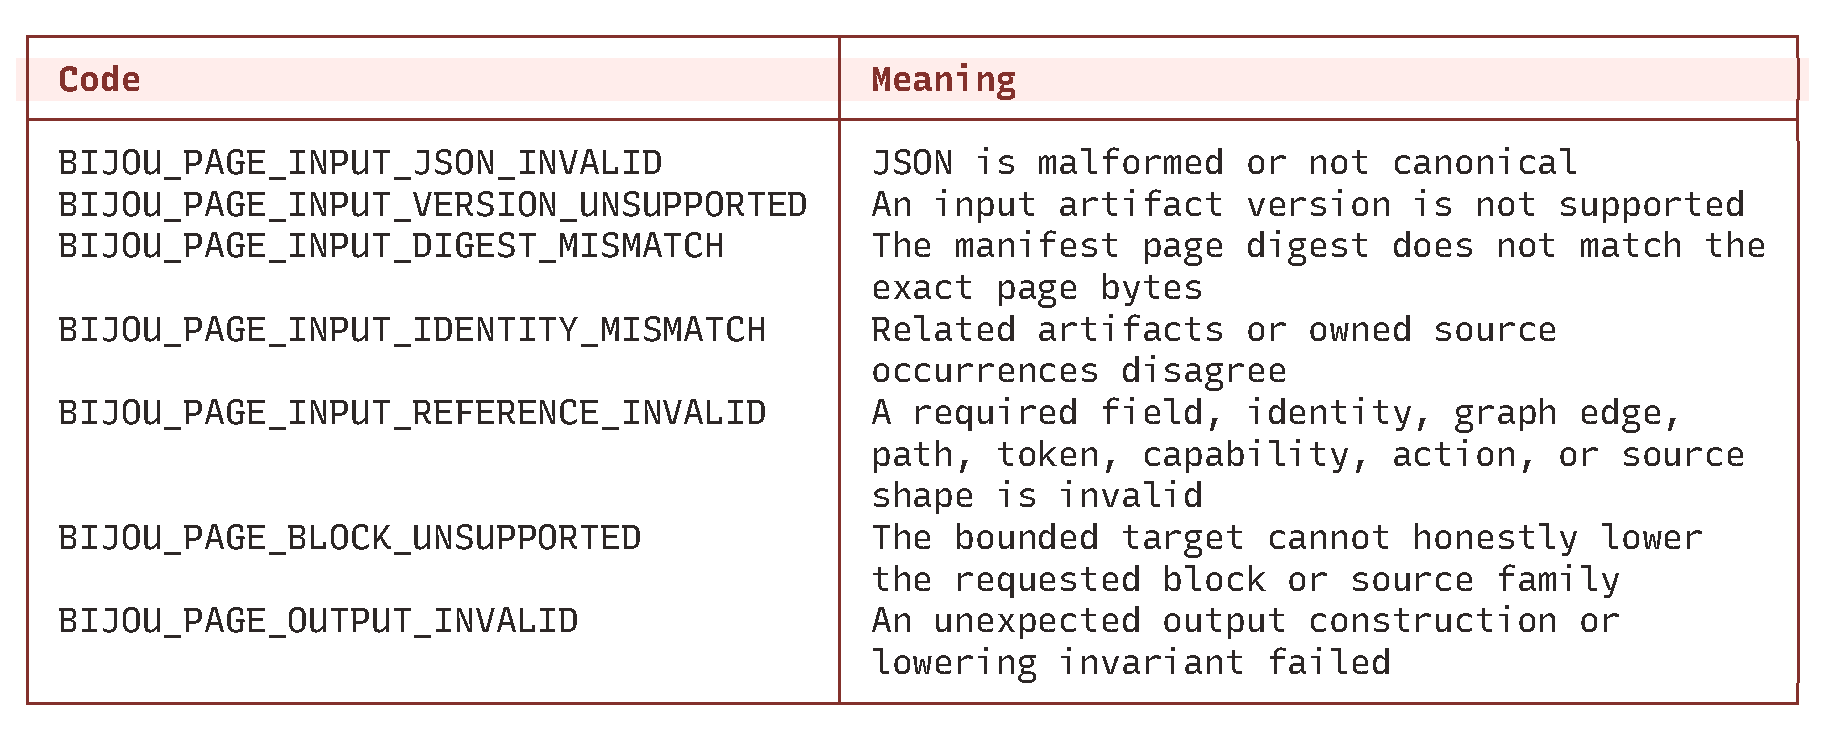
\includegraphics[width=\linewidth]{figures/tables/table-015-g1-1.pdf}
\par\smallskip{\scriptsize\color{BookMuted}Rows 1–7. Actual Bijou table component.}
\end{center}


\section{Canonical Fixture And Verification}\label{record-025-canonical-fixture-and-verification}

The checked Keep fixture pins the website-owned input bytes and the Bijou-owned outputs:

\begin{itemize}
\tightlist
\item
  \href{https://github.com/flyingrobots/bijou/blob/cbd70612140e7a450d764b3c7be1c6af878b99bc/fixtures/profunctor-page/project-keep/README.md}{Keep Profunctor Page conformance fixture}
\item
  \href{https://github.com/flyingrobots/bijou/blob/cbd70612140e7a450d764b3c7be1c6af878b99bc/docs/design/DX-050-profunctor-page-inspection.md}{DX-050 design record}
\end{itemize}

Regenerate the output artifacts:

\begin{CodeBlock}
npm run generate:profunctor-page-target
\end{CodeBlock}

Verify that the checked artifacts match the current lowerer:

\begin{CodeBlock}
npm run check:profunctor-page-target
\end{CodeBlock}

Run the focused contract evidence:

\begin{CodeBlock}
npx vitest run \
  tests/cycles/DX-050/profunctor-page-target.part01.test.ts \
  tests/cycles/DX-050/profunctor-page-target.part02.test.ts \
  tests/cycles/DX-050/profunctor-page-target.part03.test.ts \
  tests/cycles/DX-050/profunctor-page-target.part04.test.ts \
  tests/cycles/DX-050/profunctor-page-target.part05.test.ts
\end{CodeBlock}

